\section{Controllore}
Il problema della scelta del controllore è stato risolto mediante l'utilizzo dell'assegnazione degli autovalori ottenuti tramite retroazione dello stato; si affronta quindi un problema di regolazione: il moto del sistema è composto completamente dal moto libero che si vuole controllare e annullare in un tempo a piacere. Il posizionamento dei poli, e quindi la scelta del guadagno del regolatore, va eseguita sul solo sistema lineare:
\begin{figure}[H]
	\centering   	
	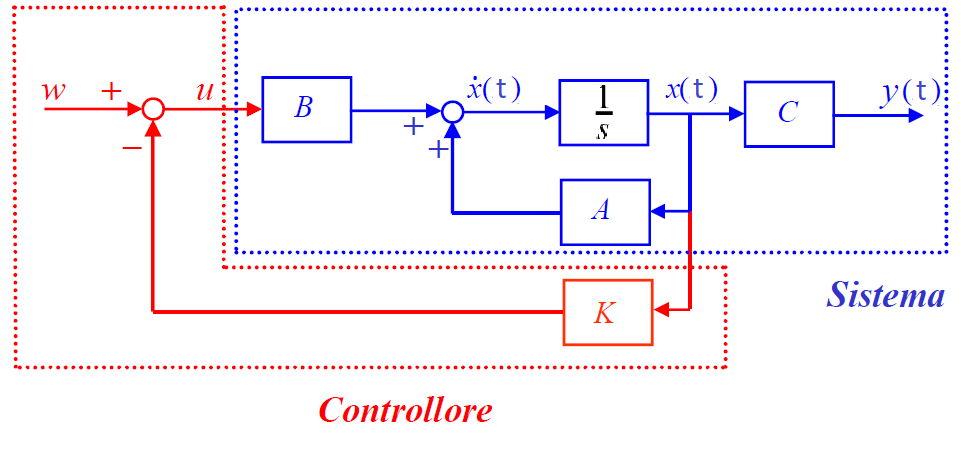
\includegraphics[width=0.70\textwidth]{Immagini/feedback_state.png}
	\caption{Schema concettuale del controllo,\cite{feedback_state}}
	\label{fig:feedback_state}
\end{figure}
Ciò che si nota in Fig.\ref{fig:feedback_state} può essere riscritto matematicamente:
\begin{center}
	$$
	\begin{cases}
	\begin{array}{c}
	x\left(t\right)=Ax{\left(t\right)}+Bu\left(t\right)\\
	y{\left(t\right)}=Cx{\left(t\right)}+Du\left(t\right)
	\end{array}
	\end{cases}
	$$
	$$
	u{\left(t\right)}=-Kx{\left(t\right)}+w{\left(t\right)}	
	$$
\end{center}Dunque:
\begin{center}
	
	$$
	x{\left(t\right)}=Ax{\left(t\right)}+Bu{\left(t\right)}=Ax{\left(t\right)}+B{\left(-Kx{\left(t\right)}+w{\left(t\right)}\right)}
	$$
	$$
	=Ax{\left(t\right)}-BKx{\left(t\right)}+Bw\left(t\right)={\left(A-BK\right)}x{\left(t\right)}+Bw{\left(t\right)}
	$$
	$$
	A_{closedloop} =A-BK
	$$
\end{center}
Per scegliere il valore di guadagno del controllore, è necessario scegliere la posizione desiderata dei poli:
\begin{center}
	$$
	G{\left(S\right)}=\frac{\omega {\;}_n^{2\;} }{s^2 +2\xi \omega {\;}_n s+\omega {\;}_n^{2\;} }
	$$
\end{center}
\begin{center}
	in cui:
	$$
	\xi =0\ldotp 7
	$$
	$$
	\omega {\;}_{n\;} =2\bullet \pi \bullet f_{\mathrm{propria}}
	$$
\end{center}Dovendo posizionare due coppie di poli complessi coniugati si sono scelte due frequenze ad una decade di distanza
\begin{center}
	
	$$
	f_{\mathrm{propria\theta}} =  0.2
	$$
	$$
	f_{\mathrm{propria\phi}} =  0.02
	$$
\end{center}Per motivi esterni il motore ha una coppia massima molto limitata ed è stato dunque necessario posizionare i poli in modo che non fossero troppo veloci.
\begin{center}
	
	$$
	polo_{\theta} = \left(\begin{array}{c}
	-\frac{7\,\pi }{250}+\frac{\pi \,\sqrt{51}\,\mathrm{i}}{250}\\
	-\frac{7\,\pi }{250}-\frac{\pi \,\sqrt{51}\,\mathrm{i}}{250}
	\end{array}\right)
	$$
	$$
	polo_{\phi} = \left(\begin{array}{c}
	-\frac{7\,\pi }{25}+\frac{\pi \,\sqrt{51}\,\mathrm{i}}{25}\\
	-\frac{7\,\pi }{25}-\frac{\pi \,\sqrt{51}\,\mathrm{i}}{25}
	\end{array}\right)
	$$
\end{center}	Questi quattro poli si può notare che abbiano parte reale negativa; la stabilità in questo modo è raggiunta.\\
Con il comando \textit{place} di Matlab si ottine dunque:
\begin{center}
	
	$	K =[  -0.0023  , -0.0278, -28.1397  , -7.7022]$
	
\end{center}
Il sistema in anello chiuso ha i seguenti poli:
\begin{figure}[H]
	\centering   	
	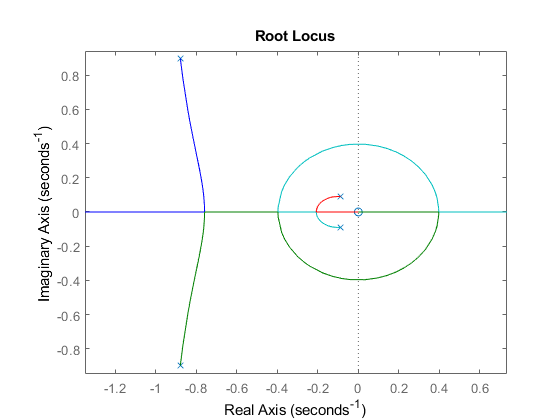
\includegraphics[width=1\textwidth]{Immagini/root_locus_closed_loop.png}
	\caption{Root locus del sistema in anello chiuso}
	\label{fig:closed_loop_root}
\end{figure}
Si va ora ad analizzare la risposta del sistema al controllo ottenuto nei punti precedenti, per assicurarci, che quanto scritto sopra valga oltre che nella teoria anche nella pratica:
\begin{figure}[H]
	\centering   	
	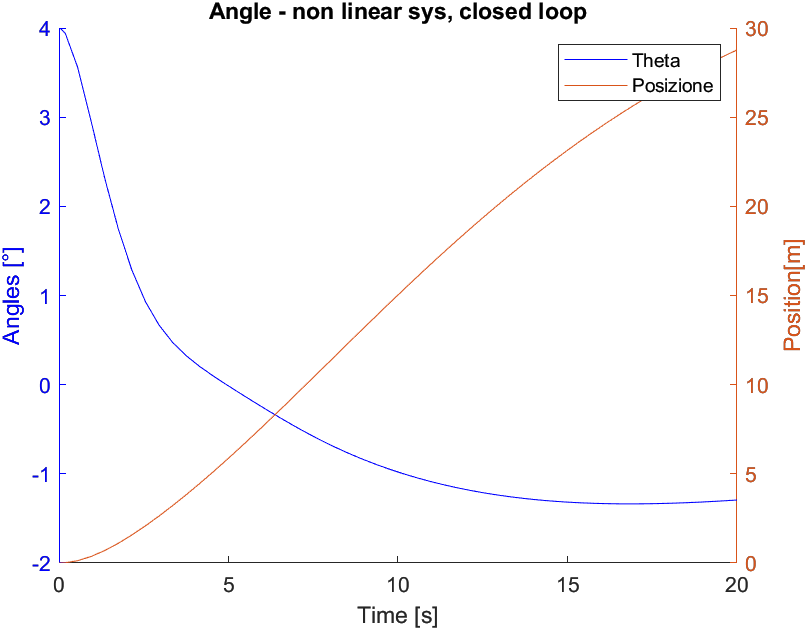
\includegraphics[width=0.7\textwidth]{Immagini/closed_loop_non_linear.png}
	\caption{Risposta del sistema non lineare in anello chiuso}
	\label{fig:closed_loop_non_linear_response}
\end{figure}
\begin{figure}[H]
	\centering   	
	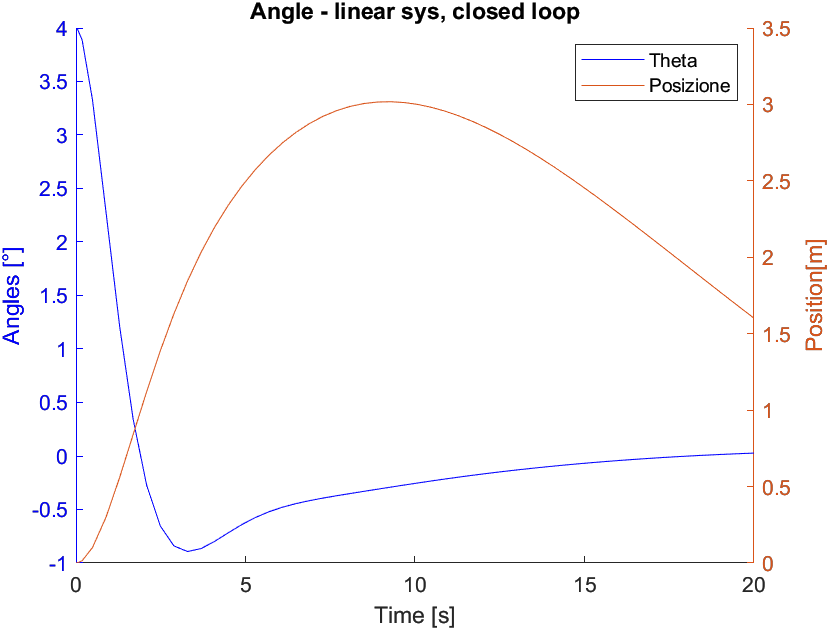
\includegraphics[width=0.7\textwidth]{Immagini/closed_loop_linear.png}
	\caption{Risposta del sistema lineare in anello chiuso}
	\label{fig:closed_loop_non_linear_response}
\end{figure}
TODO: come spieghiamo la differenza? rifare la simulazione?

\chapter{OPC - UA}
Per quanto riguarda la parte di controllo, il sistema presenta un articolato insieme di controllori inter-operanti tra di loro: nello specifico ad ogni singolo controllore sono affidate delle mansioni ben specifiche, tutte ovviamente volte al controllo e alla stabilizzazione del \textit{veicolo auto bilanciato}.

In questa fase dello sviluppo del progetto, siamo andati ad implementare parte del codice che verrà installato, in un secondo momento, a bordo del raspberry: esso infatti svolge, all'interno del sistema (come si vede in figura ~\ref{fig:OPCUA_schema}) una comunicazione a due direzioni, che ne determinano due comportamenti differenti:
\begin{itemize}
	\item Come \textbf{server} per la parte di comunicazione \textit{OPC-UA} (per il settaggio dei guadagni);
	\item Come \textbf{master} nella comunicazione seriale verso Arduino (per quanto riguarda invece la gestione dell'algoritmo di controllo);
\end{itemize}

 \begin{figure}[H]
	\centering   	
	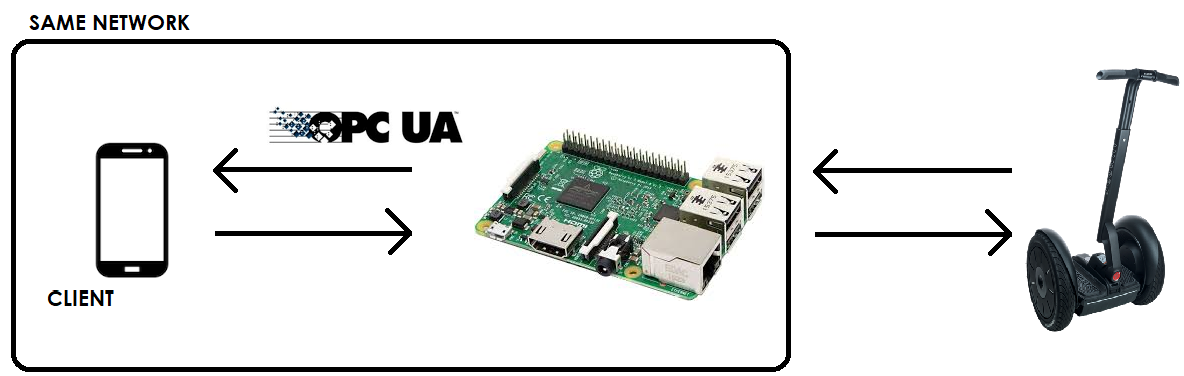
\includegraphics[width=0.75\textwidth]{Immagini/OPCUA_schema.png}
	\caption{Schema di massima dell'utilizzo di Raspberry Pi 3}
	\label{fig:OPCUA_schema}
\end{figure}

In questa fase abbiamo quindi sviluppato la parte relativa all'utilizzo di \textit{Raspberry Pi 3} come \textit{server OPCUA}.

\section{Idea base OPC-UA}
L'\textit{Open Platform Communications Unified Architecture} (OPC UA) è un protocollo di comunicazione automatico per l'automazione industriale. 

OPC UA sostituisce il protocollo \textit{OPC Classic}, conservando tutte le funzionalità del predecessore. Poiché OPC Classic era stato costruito su una tecnologia Microsoft detta modello a oggetti per componenti distribuiti, era vincolato a Microsoft, ma questa caratteristica è diventata sempre più limitante.

OPC UA risulta completamente interoperabile tra i diversi sistemi operativi usati, aggiungendosi a Windows e alle tecnologie industriali come i PLC, inoltre comprende Linux, iOS e anche sistemi operativi per dispositivi mobili come Android. Consentire al maggior numero di dispositivi possibile di comunicare contribuisce al progresso dell'IoT.

Queste caratteristiche di \textbf{interoperabilità} sono state sfruttate al massimo in questo contesto, potendo così creare, in maniera semplice e veloce, una comunicazione tra differenti tipologie e famiglie di dispositivi.

\section{OPC-UA e V.A.B.}
Nel contesto del progetto del \textit{veicolo auto bilanciato}, siamo andati ad utilizzare il protocollo di comunicazione \textit{OPC-UA} come supporto per il tuning dei parametri relativi al \textbf{gain} del controllore, ovvero ai parametri del vettore \textit{K}, che abbiamo chiamato (all'interno dello script di Python):
\begin{itemize}
	\item \textbf{K\_phi}
	\item \textbf{K\_phi\_p}
	\item \textbf{K\_theta}
	\item \textbf{K\_theta\_p}
\end{itemize}

Nello specifico, lo scambio di parametri tra server e controllore avviene tramite unfile \textit{.txt}, che permette, in maniera semplice e immediata, di implementare uno scambio di informazioni tra il server \textit{OPC-UA} strutturato in Python e l'ambiente \textit{real-time} introdotto a bordo del controllore \textit{Raspbery Pi 3}.


In particolare abbiamo due files:
\begin{itemize}
	\item \textbf{Un file temporaneo} \textit{("GainParametersToController.txt")} utilizzato come pipeline per il passaggio dei parametri tra server e controllore. Questo risulta essere un file temporaneo che viene ad essere cancellato e ricreato ogni qualvolta che il server viene spento e successivamente riaccesso.
	Nello specifico, ad ogni riaccensione, i valori iniziali di questo file, vengono settati con gli stessi valori presenti nel file \textit{definitivo}  (qualora quest'ultimo esista già: in caso contrario si procede con un inizializzazione dei parametri a 0);
	
	\item \textbf{Un file definitivo} \textit{("GainParametersConfirmed.txt")} il quale invece viene creato una e una sola volta e sul quale poi vengono salvati i parametri che saranno poi letti all'accensione successiva del server ed utilizzati come parametri iniziali per il controllore.
\end{itemize}

Questi file possono essere settati con i parametri presenti nel server che sono visibili in figura ~\ref{fig:OPCUA_params}, nello specifico:
\begin{itemize}
	\item \textbf{Submit change to controller} permette di scrivere i valori dei gains sul file \textit{"GainParametersToController.txt"};
	
	\item \textbf{Store definitively in file} permette di scrivere i valori dei gains sul file \textit{"GainParametersConfirmed.txt"};
	
	\item \textbf{SHUT DOWN SERVER} permette invece di spegnere il server e di cancellare successivamente il file temporaneo.
\end{itemize}

\begin{figure}[h]
	\centering   	
	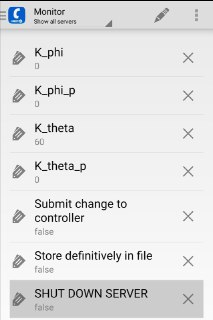
\includegraphics[width=0.4\textwidth]{Immagini/OPC_UA_params.jpg}
	\caption{Parametri impostabili lato client}
	\label{fig:OPCUA_params}
\end{figure}


Abbiamo racchiuso in figura ~\ref{fig:OPCUA_diagram} il funzionamento di massima del codice lato server: codice che siamo andati a testare utilizzando un'apposita app per smartphone Android (\href{https://play.google.com/store/apps/details?id=com.prosysopc.ua.android2&hl=it}{OPC-UA Android client}).

\begin{figure}[h]
	\centering   	
	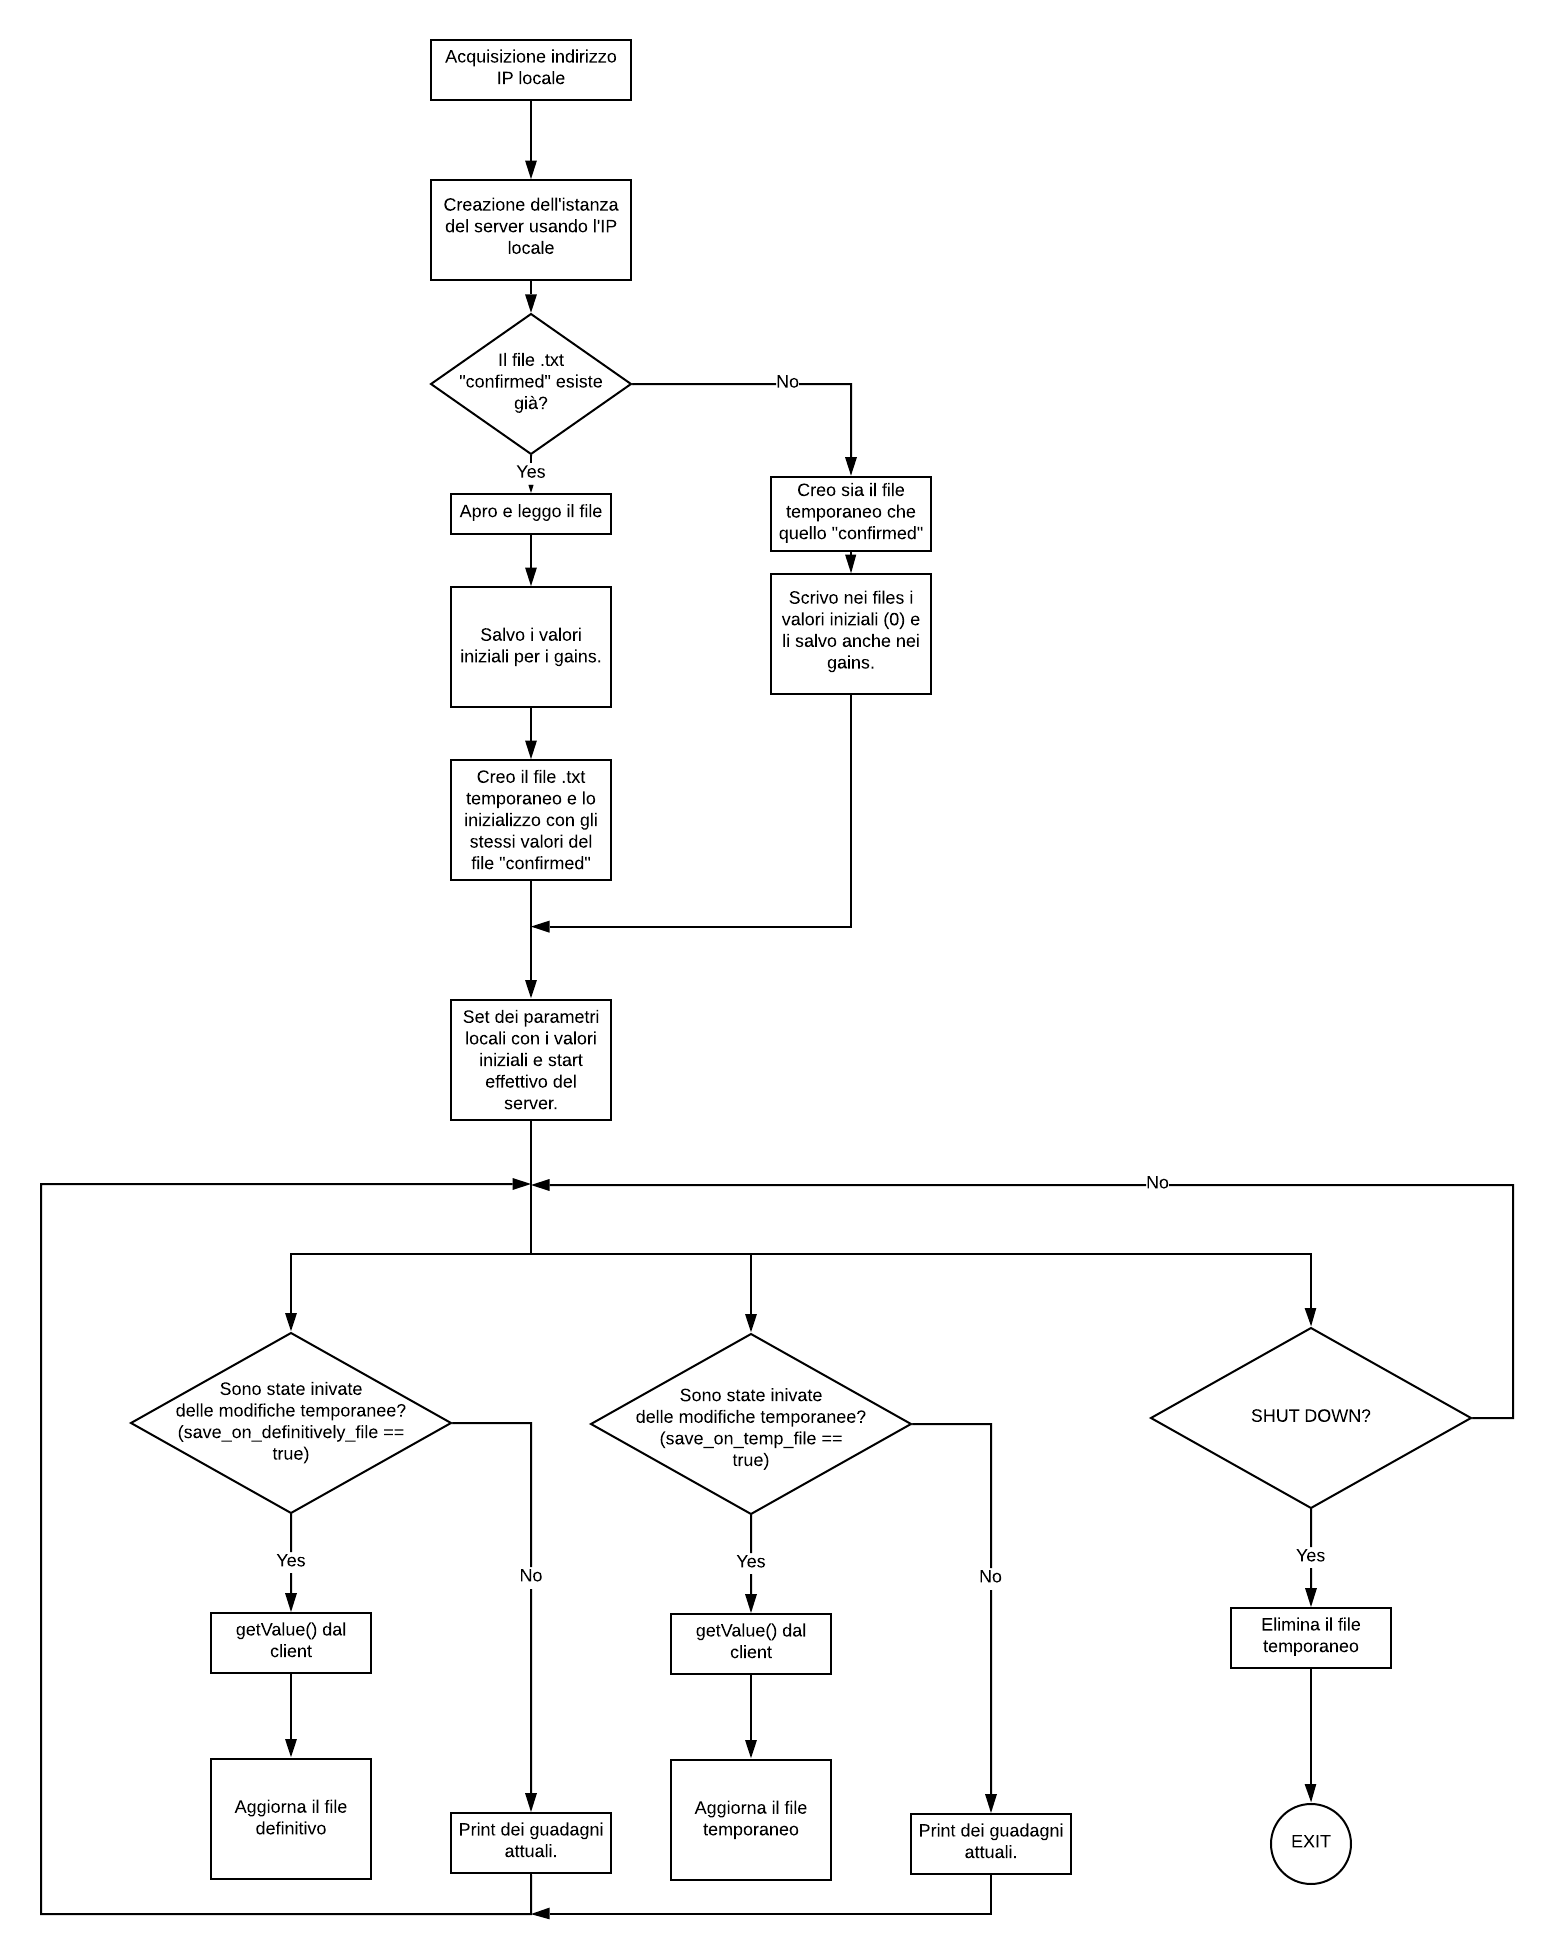
\includegraphics[width=0.7\textwidth]{Immagini/OPCUA_diagram.jpeg}
	\caption{Diagramma rappresentante le funzionalità del server}
	\label{fig:OPCUA_diagram}
\end{figure}

\chapter{Rumore}
Piattaforma inerziale --> PSD
Questione anti windup --> coppia già limitata quindi nessun vincolo di saturazione